% Chapter4
\chapter{Implementierung} \label{chapter:thevetestcase}
\section{Modellierung der Anlage}
Für das Aufbauen einer Anlage, ist ein vorab überlegtes Konzept von großer Bedeutung. Mittels des Rohr- \& Instrumentenfließschemas wird ein später noch des öfteren abgeändertes Abbild erstellt. Die in der Anfangsphase aufkommenden Änderungen ergeben sich angesichts der nur partiellen Implementierung der Anforderungen. Initial wird hoher Wert auf Redundanzen gelegt. Erst eine größere Anzahl an Bauteilen kann einen parallelen Ablauf mehrerer Arbeitsschritte ermöglichen. Durch die drei eingebauten Tanks und zwei Reaktoren, die mittels der drei Hauptleitungen verbunden sind, ist das Umfüllen zwischen zwei Tanks, sowie das gleichzeitige Befördern von Flüssigkeit vom dritten Tank in einen der Reaktoren möglich.\\

Die zwei Pumpen sind so platziert, dass bei einem eventuell auftretenden Defekt die andere Pumpe deren Aufgabe übernehmen kann. Arbeitsschritte können dadurch zwar nur noch sequentiell abgearbeitet werden, jedoch kommt es nicht gleich zu einem totalen Ausfall der Funktionalität der Anlage. Eine weitere Absicherung gegen möglich aufkommende Störfälle ist die Position der Tanks. Durch ihre Lokalisation an der höchsten Stelle der Apparatur besteht die Opportunität die Schwerkraft zu nutzen.\\

\begin{figure}[h!]
  \centering
  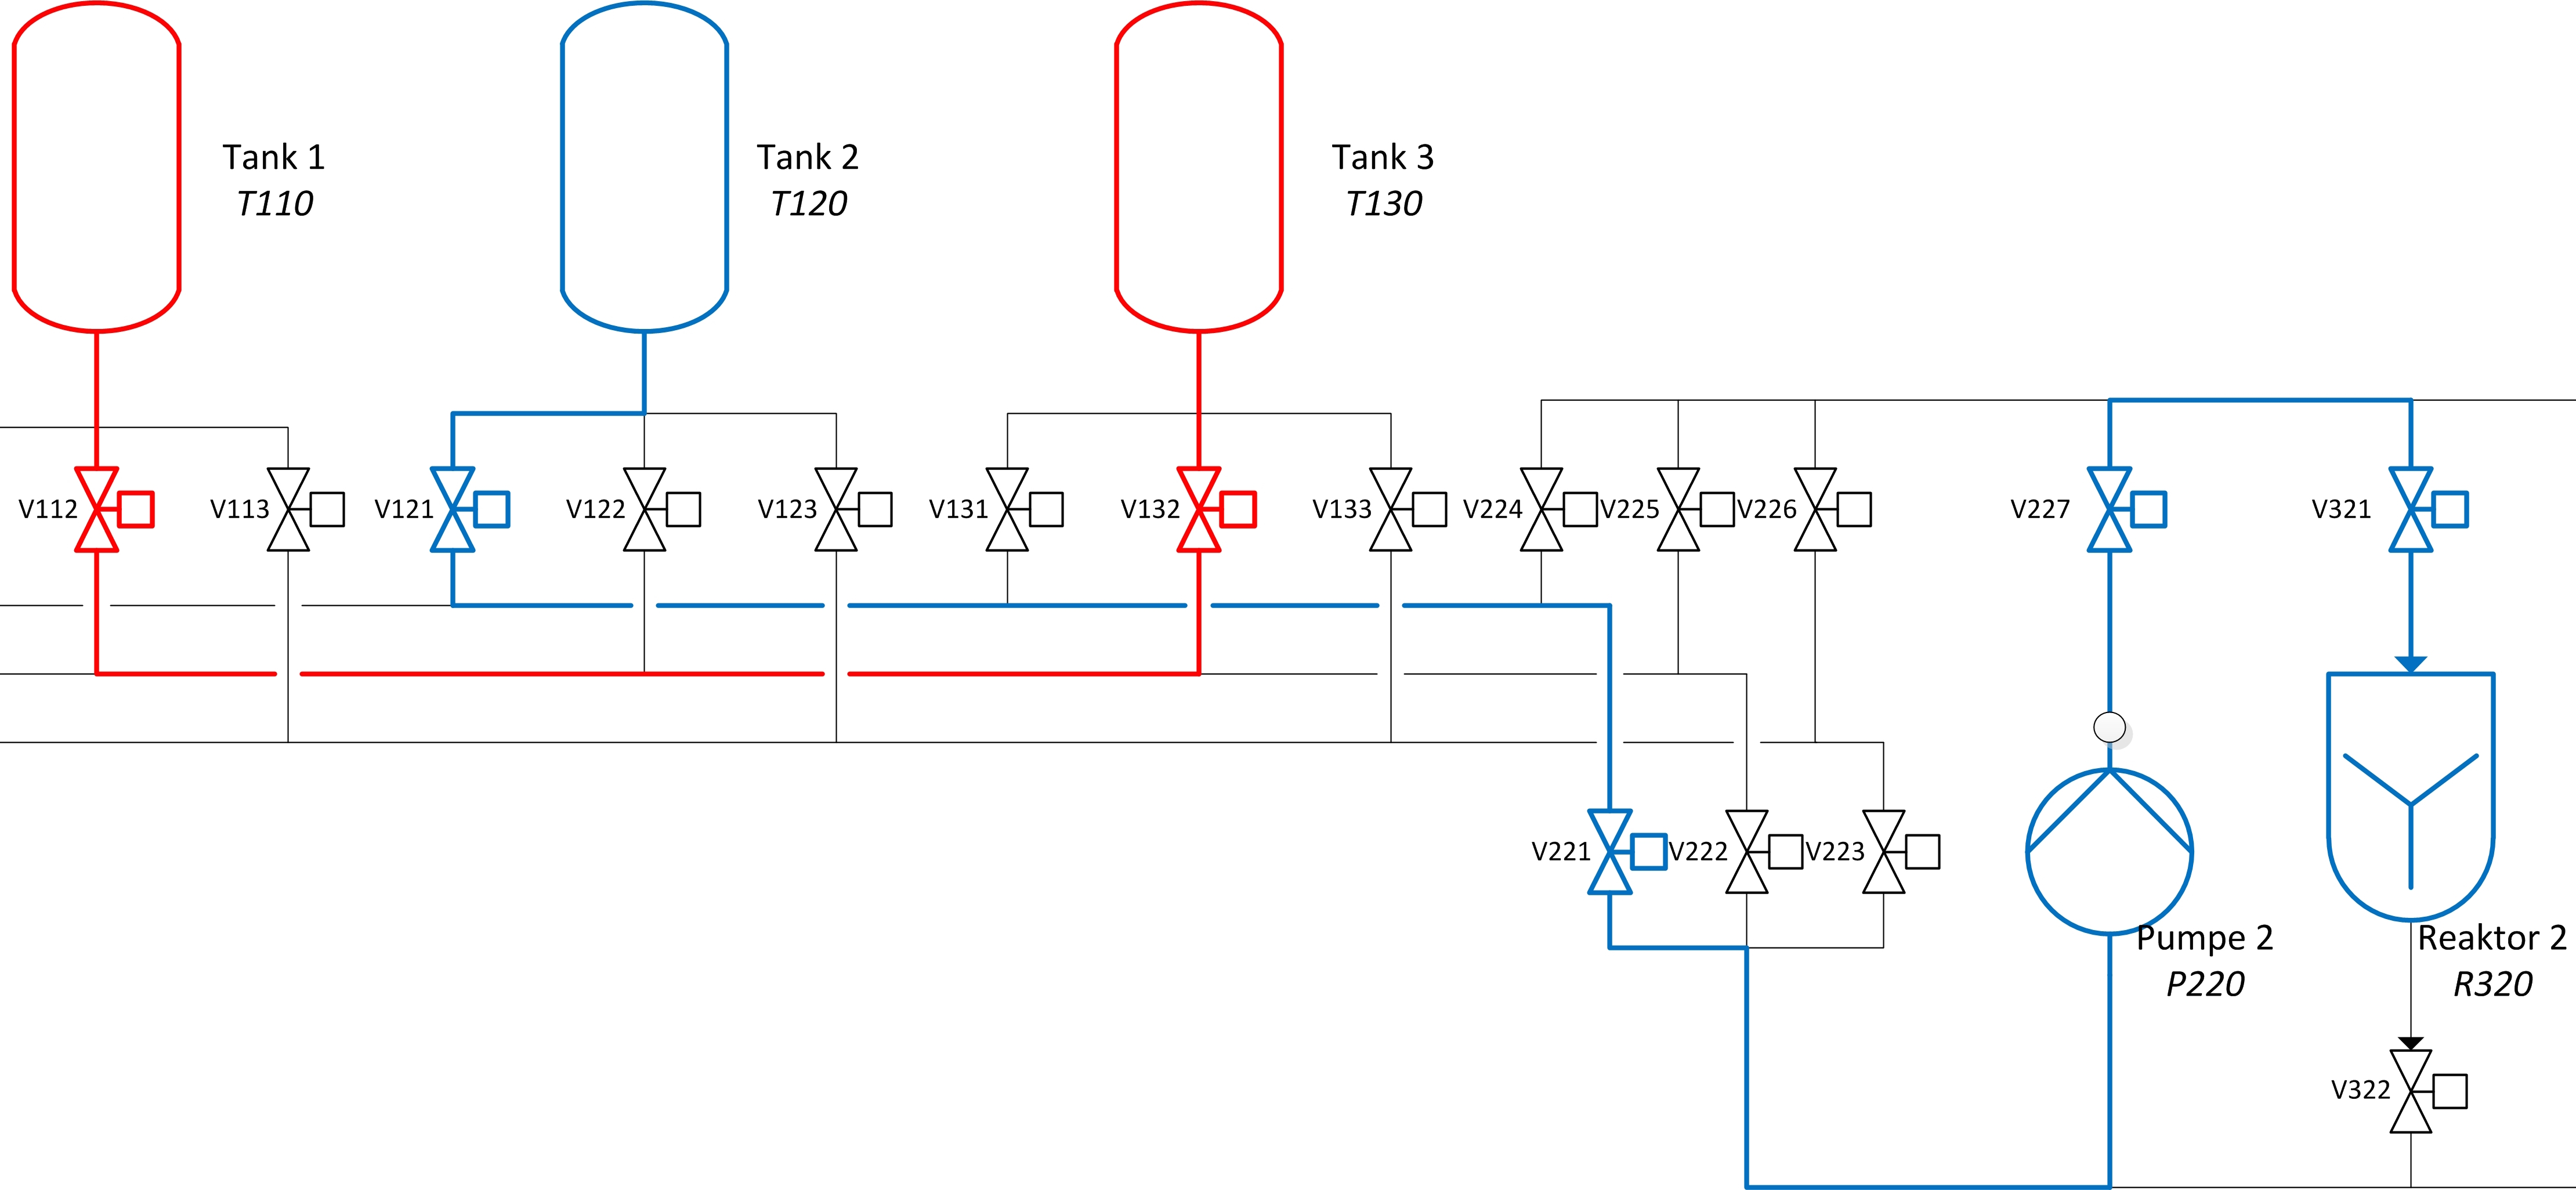
\includegraphics[width=1\textwidth]{graphics/implementation/RI_Impl_cropped.jpg}
  \caption{Mögliche Parallelität im RI ersichtlich}
\end{figure}

Jedes Ventil hat eine vorteilhafte Durchflussrichtung, die meistens mit einem Pfeil direkt auf dem Bauteil gekennzeichnet ist. Ganz abgesehen davon, ob es sich um ein Ventil handelt, welches im stromlosen Zustand geschlossen ist oder ob es ein schließendes Ventil ist, diese Vorgabe sollte stets eingehalten werden. Aspekte wie dieser haben in die Modellierung der Anlage selbstverständlich eingebaut zu werden.\\

\todo[inline]{BILD EINFÜGEN}

\begin{figure}[h!]
  \centering
  %\includegraphics[width=0.7\textwidth]{graphics/implementation/BILD}
  \caption{Ventil mit vorteilhafter Fließrichtung}
\end{figure}

Um in der Anlage befindliche Flüssigkeiten zu entfernen muss ein eigens für den Auslass vorgesehenes Ventil installiert werden. Vorteilhafterweise handelt es sich bei der Position dieses Bauteils um den tiefsten Punkt der Apperatur. Alternativ dazu kann dieses auch direkt nach einer Pumpe montiert werden.

\section{Aufbau der Anlage}
\section{Phasen und Rezepte}
\section{HMI}
Für dieses Projekt wurde als SCADA System die Software zenon vorgegeben, daher wird das HMI in zenon Supervisor (zenons HMI Programm) umgesetzt.\\
\\
\textbf{Visualisierung}\\
In zenon wird eine Visualisierung \glqq Bild\grqq\space  gennant. Dieses kann mit vorgefertigten Elementen erweitert werden. 

Als Ausgangspunkt für die Visualisierung wurde das RI-Fließeschema zur Hand genommen. Aus diesem wurde die Anzahl der Elemente und die Grundstruktur übernommen. Als nächsten Schritt musste evaluiert werden, welche Inhalte des RI-Fließschemas für die Visualisierung relevant und welche Informationen nicht vorhanden waren.\\
\\
\textbf{Feldbuskonfiguration}\\
Um eine Visualisierung mit aktuellen Sensorwerten zu befüllen, wird eine Verbindung zur SPS benötigt. Diese Verbindung wird über das Teilprogramm zenon Logic (im weiteren nur noch Logic genannt) hergestellt.\\
\\
Als ersten Schritt, um in Logic eine SPS hinzuzufügen, muss im Unterpunkt \glqq Feldbuskonfiguration\grqq\space die Treibersoftware für die ADAM5550 SPS hinzugefügt werden. Daraufhin müssen alle Module, die an der SPS angebracht sind, in die Konfiguration hinzugefügt werden.\\%todo Position
\begin{figure}[h!]
  \centering
  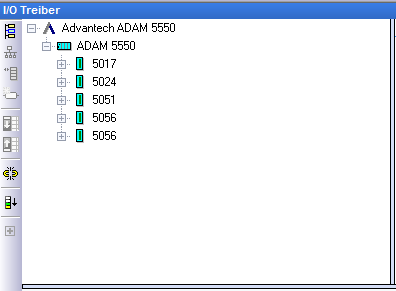
\includegraphics[width=0.7\textwidth]{graphics/implementation/Feldbuskonfiguration}
  \caption{Feldbuskonfiguration}%todo Grafik name
\end{figure}
\\
\textbf{Variablen}\\
In zenon können auf mehrere Arten Variablen erstellt werden. Damit diese für die Visualisierung und von Logic sichtbar sind, müssen sie als Globale Variable definiert werden. Der einfachste Weg dafür ist es, im Logic Variablenfenster, über den Reiter  \glqq Globale Variablen\grqq, die Funktion \glqq Variable hinzufügen\grqq\space aufzurufen.\\%todo Position
\begin{figure}[h!]
  \centering
  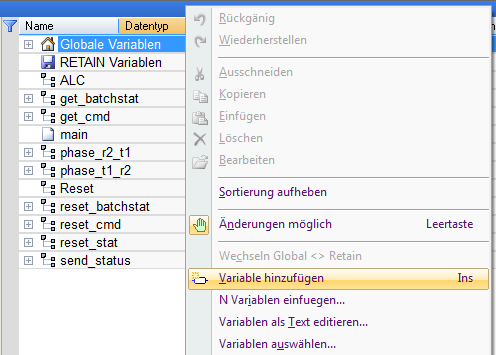
\includegraphics[width=0.7\textwidth]{graphics/implementation/Variablen}
  \caption{Variablen}%todo Grafik name
\end{figure}\\
Sobald alle Variablen erstellt sind, werden diese mit der Feldbuskonfiguration verknüpft. Durch diesen Schritt erhält man Zugang zu den an der SPS angeschlossenen Bauteilen.\\
%Die erstellten Variablen mussten als nächstes in der Visualisierung eingetragen werden um in dieser im nächsten Schritt eine Steuerung zu erzeugen.\\
\\
%Feldbuskonfiguration -> Konfiguration einfügen (Advantech ADAM 5550) -> Master/Port hinzufügen (ADAM 5550) -> Slave/Datenblock einfügen (Slot:Steckplatz an SPS; Module: Analog/Digital|In/Out|4/8/16 Channels...) -> Variable hinzufügen (Channel; Variablenname)
%Variable -> Globale Variable hinzufügen (erzeugt Variable in logic und auch im supervisor zugänglich für die Visualisierung) -> In Visualisierung zu den Elemente die richtigen Variablen hinzufügen -> Bei Feldbbuskonfiguration bei richtiger I/O auf richtigem Channel hinzufügen
%TEST -> logic Programm hochladen -> Variablen in logic zeigen aktuelle werte an -> check mit werten direkt von der SPS

%Umrechnen von Sensorwerten: 
%Durchflusssensor Digital -> etwa 900 ticks pro Liter -> Timer bid 900 ticks -> Liter/min
%Füllstandsensor 4-20mA -> 4=voll, 20=leer -> Variablen/Tank Konfiguration -> Umrechnung 4=100, 20=0
%Ventilstatus 0/1 -> Variablen Konfiguration -> Extremwerte farblich markieren -> Ventil Elementfarbe nach Variablen Farbe
\textbf{Steuerung}\\
\\
Phase 1 Steuerung mittels Buttons\\
	Der erste Versuch war es die Steuerung mittels einfachen Buttons umzusetzen. Diese haben meist die in zenon vorhandene Funktion  \glqq Sollwert absetzen\grqq\space  verwendet, welche den Wert einer Variable ändert.\\
	So konnten alle Funktionen umgesetzt werden, dadurch erhielt das  \glqq Bild\grqq\space  jedoch viele Elemente die von der Eigentlichen Visualisierung ablenkten.\\
\\
Phase 2 Versteckte Buttons\\
	Um den Element-Overload zu verringern war der nächste Schritt die Button zu  \glqq verstecken\grqq\space  indem sie Transparent über die eigentlichen Elementen (beispielsweise ein Ventil) verschoben wurden.\\
	In der Visualisierung wurden nun weniger  \glqq unwichtige\grqq\space  Bausteine angezeigt, die Elemente waren jedoch immer noch da, wodurch die Größe (MB) der Visualisierung deutlich anstieg.\\
\\
Phase 3 Funktionale Elemente\\
	Der nächste schritt war es die nicht funktionalen Grafikelemente durch Buttons in Form der gewünschten Elemente zu ersetzten.\\
\\
\textbf{Rezepterstellung}\\

\section{Ontology}
Nachdem die Evaluierung der wichtigsten Aspekte im Kapitel Ontologie der Chargenprozessanlage in Hinsicht auf eine automatisierte Codegenerierung durchgeführt wurden, behandelt dieses Kapitel den Werdegang der Ontologie vom Ersten bis hin zum Finalem Design.\\
\\
Das Ziel der Ontologie ist es, die im laufe dieses Projekts aufgebaute Anlage in einer Art und Weise abbilden zu können, die es erlaubt daraus eine automatisierte Codegenerierung durchzuführen und dabei auf einem Abstraktionslevel zu bleiben um einen Großteil an in der Industrie vorkommenden Produktionsanlagen abbilden zu können.\\
\\
Da es den Rahmen dieser Arbeit sprengen würde, auf jeden einzelnen Gedankengang in der Erstellung der Ontologie einzugehen, werden nur die großen Revisionen der Ontologie genauer beschrieben.

\begin{figure}[hbt!]
  \centering
  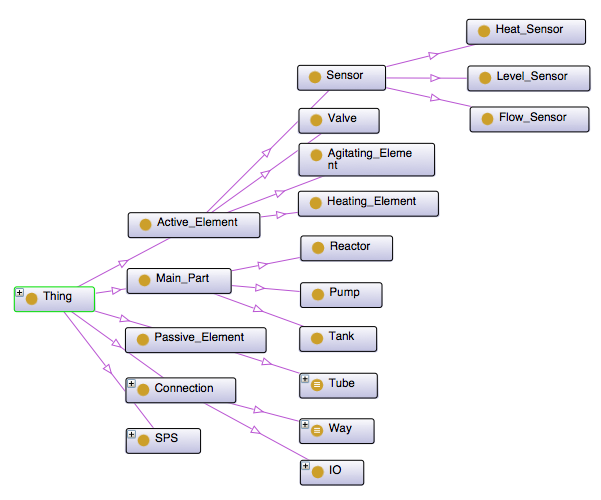
\includegraphics[width=0.6\textwidth]{graphics/implementation/Ontology_v2}
  \caption{Erste Revision der Ontologie}
\end{figure}

In der Anlage gibt es verschiedene Arten von Bauteilen: Sensoren, Aktuatoren, Tanks, etc., daher haben wir diese in der Ontologie in folgende Kategorien unterteilt.\\

Main\_Part: Dies sind alle Elemente die subjektiv als Hauptelemente bezeichnet sind.\\
Active\_Element: Jene Bauteile die etwas tun - Aktuatoren, Sensoren\\
Connection: Verbindungen zwischen den einzelnen Bauteilen\\
Passive\_Elements: In der Anlage verbaute teile die keine Arbeit verrichten.\\ 
\\
Mit dieser Ontologie ist es grundsätzlich möglich die Anlage aus Kapitel 4.2 abzubilden, jedoch finden sich einige Inkonsistenzen die die automatisierte Codegenerierung erschweren wenn nicht sogar unmöglich machen würden. 

\begin{figure}[hbt!]
  \centering
  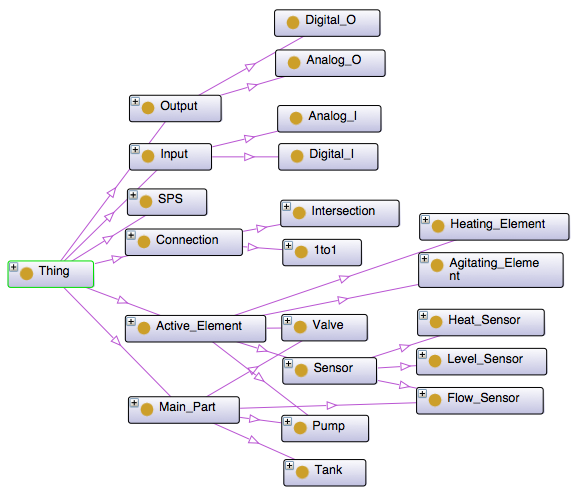
\includegraphics[width=0.6\textwidth]{graphics/implementation/Ontology_v4}
  \caption{Dritte Revision der Ontologie}
\end{figure}



\section{Aktivitätsdiagramm}
\section{Codegenerierung}

TODO